% \chapter{The Standard Model}
% \label{sec:01_sm}

\chapter{Introduction}
\label{sec:01_intro}

\begin{center}
	\centering
	\noindent
	\textit{God used beautiful mathematics in creating the world.} --- Paul Dirac~\cite{pagels2012cosmic}
\end{center}

\vskip0.5\baselineskip

The standard model (SM) of particle physics is perhaps the greatest scientific theory of all time.
It is a mathematical representation of three fundamental forces, all known elementary particles, and their collective interactions.
In a broader sense, it is also the culmination of centuries of iterative, syncretic experimental results and theoretical advances, from Newton's laws of motion up to the discovery of the Higgs boson.
That such a wide array of seemingly idiosyncratic physical phenomena and theories --- electricity, magnetism, radioactive decays, quantum mechanics, special relativity, the structure of the atom, the binding of the nucleus, the behavior of elementary particles, and more --- can all be encapsulated at their most primordial level into a single theory exemplifies the beauty of the SM.
% In this chapter, we
% Indeed, on a personal note, this is what has always attracted me to particle physics, and I attempt in this chapter to capture just some of the beauty of the SM.

This beauty is most apparent when viewing the SM through the lens of \textit{symmetries}.
Symmetries provide an elegant way to precisely describe the extremely complex physics mentioned above.
Indeed, superficially, the SM can be viewed simply as a classification of elementary particles and their interactions according to their behavior under different symmetries of the universe and its mathematical description.

This is illustrated in Figure~\ref{fig:01_sm}, listing the SM particles and their properties.
They are first divided into two classes, fermions and bosons, based on how they behave under Lorentz transformations --- a fundamental physical symmetry of nature.
This simple distinction has profound implications: fermions constitute matter, i.e. what all the ``stuff'' in the universe is made out of, while bosons are the particles responsible for forces and their interactions.
Specifically, the photon mediates electromagnetism, the $W^{\pm}$ and $Z$ bosons the weak force, and gluons the strong force.
There is also the Higgs boson, which is special: it does not mediate a force in the classical sense, but its interactions with elementary particles are what imbues them with mass.

\begin{figure}[ht!]
	\centering
	% \captionsetup{justification=centering}
	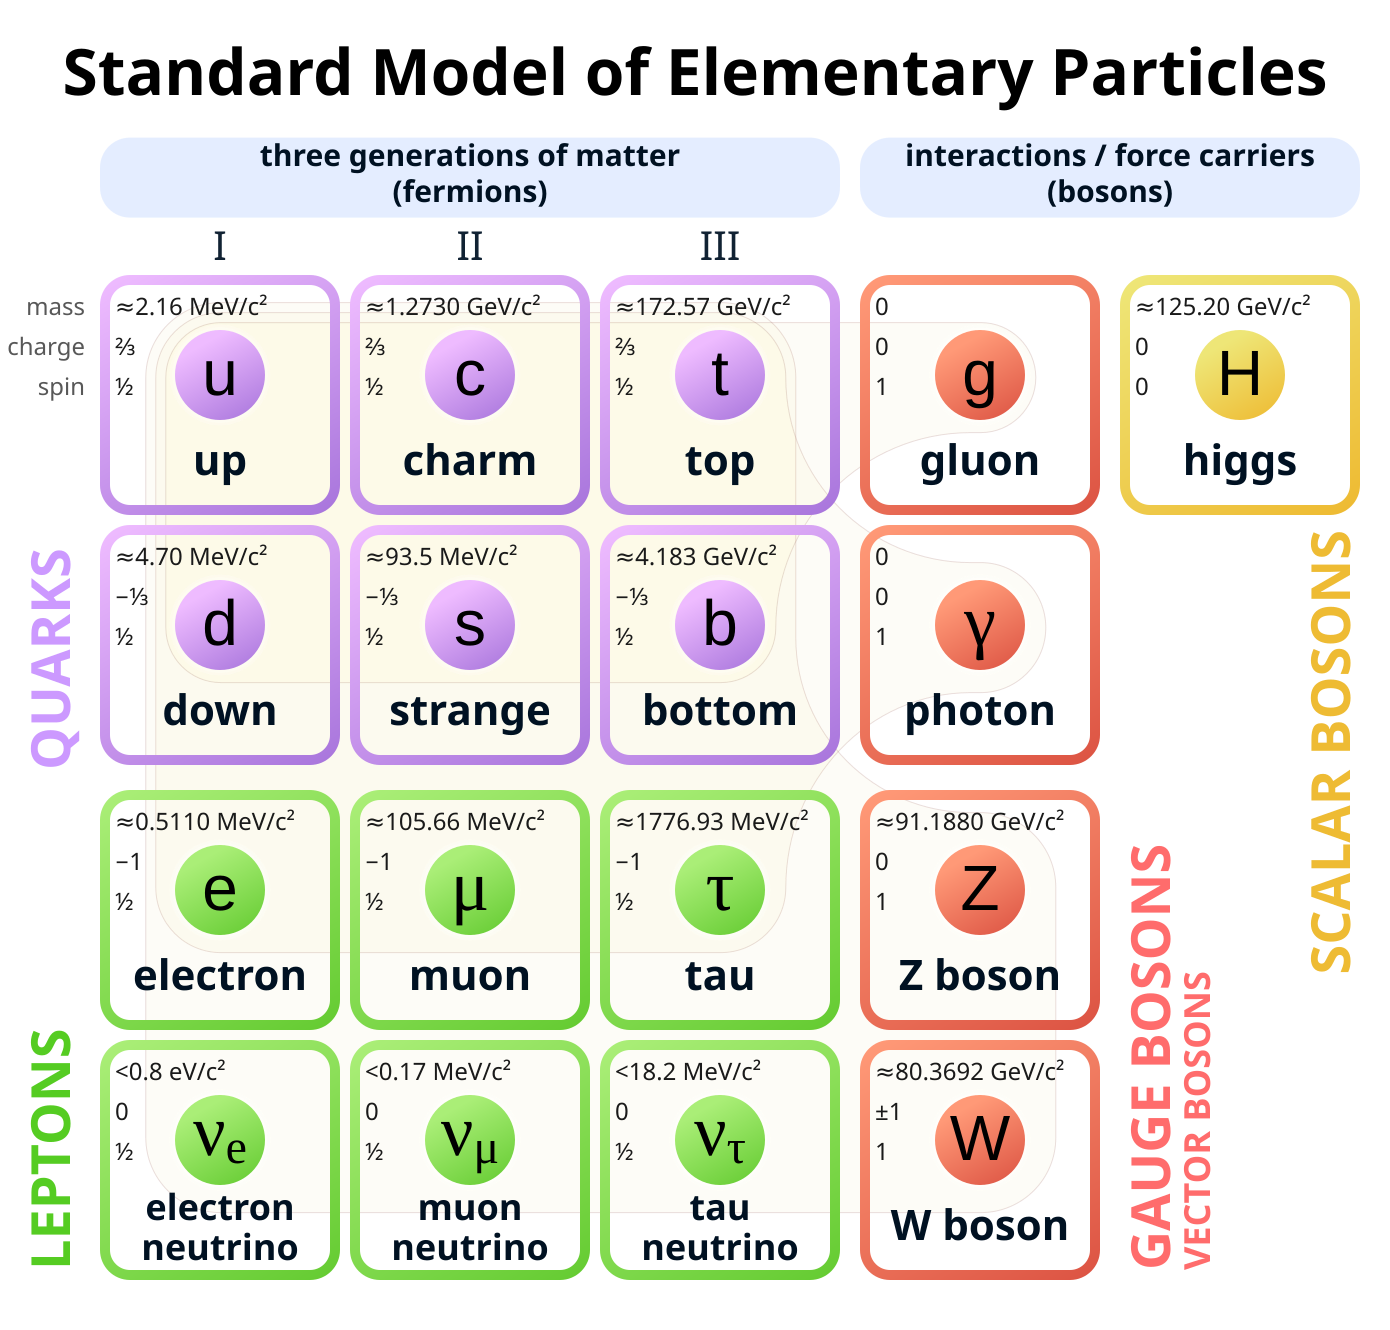
\includegraphics[width=0.8\textwidth]{figures/01-SM/sm_diagram.png}
	\caption{Particles and their classifications in the SM, reproduced from Ref.~\cite{enwiki:1238968997}.}
	\label{fig:01_sm}
\end{figure}

Each force is intimately tied to a symmetry in the SM, and particles are further distinguished by their behavior under these symmetries --- or, equivalently, how they are affected by this force.
Fermions are divided by those interacting (quarks) and not interacting (leptons) with the nuclear strong force, while each of their rows in Figure~\ref{fig:01_sm} further separates them by different ``charges'' under the weak force.
Additionally, each particle's mass and electric charge represent the strength of its interaction with the Higgs and electromagnetic fields, respectively.
Finally, we can see a mysterious \textit{almost}-symmetry: there are three copies, or ``flavors'' or ``generations'', of each fermion, which are entirely identical but for their masses (e.g. the electron, muon, and tau family of particles).
Such a structure may suggest the presence of new, yet-to-be-discovered forces tied to this symmetry.

In these notes, we aim to make this picture more precise.
The mathematical frameworks needed to do so are called group theory and quantum field theory (QFT), and are the subjects of Chapters~\ref{sec:01_symmetries} and~\ref{sec:01_qft}, respectively.
Equipped with these tools, we finally describe the SM in Chapter~\ref{sec:01_sm}, including the interactions discussed above and electroweak symmetry breaking.

These notes build off of several great resources, including:
\begin{itemize}
	\item David Tong's extremely useful and insightful lecture notes on QFT~\cite{TongQFT}, gauge theories~\cite{TongGT}, and the standard model~\cite{TongSM};
	\item John McGreevy's great course on symmetry in physics~\cite{McGreevyGT} (which I had the pleasure of attending in the Fall of 2020);
	\item Frederic Schuller's precise lectures on the geometric anatomy of theoretical physics~\cite{SchullerGATP};
	\item Tony Zee's \textit{Group Theory in a Nutshell for Physicists}~\cite{Zee:2016fuk} and \textit{Quantum Field Theory in a Nutshell}~\cite{Zee:2003mt};
	\item Peskin and Schroeder's classic \textit{An Introduction to Quantum Field Theory}~\cite{Peskin:1995ev};
	\item Gavin Salam's lectures on \textit{Elements of QCD for hadron colliders}~\cite{Salam:2010zt};
	\item and Hong Liu~\cite{LiuRQFT} and Ricardo Matheus'~\cite{MatheusQFT} clear, recorded lectures on QFT.
\end{itemize}
